<<<<<<< Updated upstream
\documentclass[a4paper]{article}

\usepackage{graphicx}
\usepackage{url}
\usepackage{tabularx}
\bibliographystyle{apacite}
\graphicspath{{../images/}}

\title{Graph Isomorphism}
\author{\textbf{maximum-solution} \\ Aliza Rafiq ar05986@st.habib.edu.pk \\ Iqra Siddiqui is06176@st.habib.edu.pk \\ Shalin Amir Ali sa06132@st.habib.edu.pk \\Fahad Ahmed Shaikh fs05847@st.habib.edu.pk \\}
\date{}

\begin{document}
\maketitle

\section{Problem Statement:}
Find if two given graphs are isomorphic and select an optimal approach on the basis of comparative analysis.
\section{Description:}
With its many practical and theoretical applications, graph isomorphism remains one of the most important efficiently unresolved problem. The problem is a computational challenge that aims to determine if two graphs are isomorphic. Two graphs are said to be isomorphic if:\\
\begin{itemize}
\item Number of vertices and edges are same\\
\item Edge connectivity is retained\\
\end{itemize}
Consider following two graphs below. Even though they look different but they are isomorphic as isomorphism is the vertex bijection that is edge preserving as can be noticed below:\\
\begin{center}
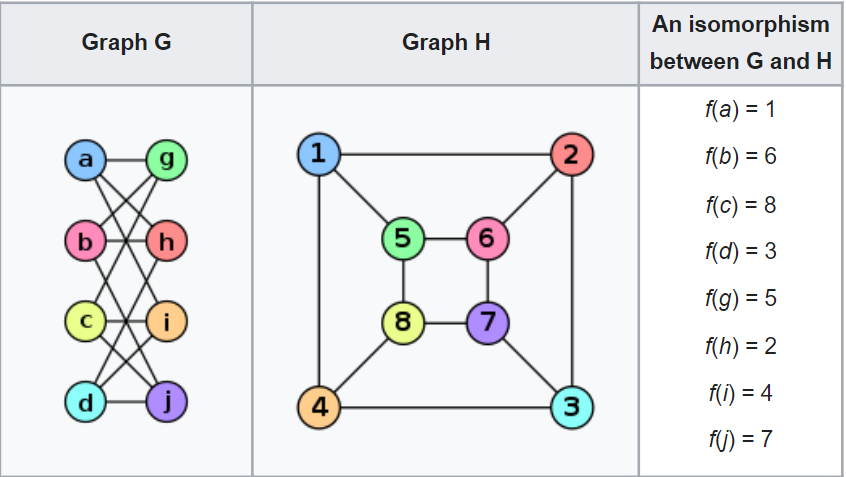
\includegraphics[width=7cm]{images/graphisomorphic.png}\\
\end{center}
Similarly in the image below, the two graphs are isomorphic as their connectivity is retained. \\
\begin{center}
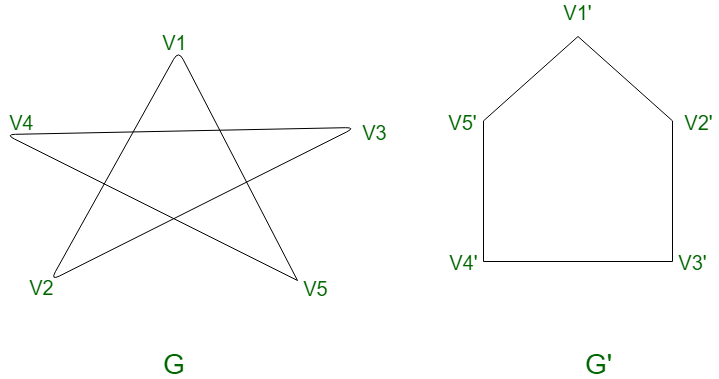
\includegraphics[width=7cm]{images/isomorphism.png}\\
\end{center}
In order to find if two graphs are isomorphic the challenge is to look for:\\
\begin{itemize}
\item Equal number of vertices \\
\item Equal number of edges\\
\item Same degree sequence\\
\item Same number of circuits of particular length\\
\end{itemize}
Hence, this problem is a NP-Intermediate problem as no current solution is known that is either NP complete or polynomial time. However for some special cases of graphs, such as trees, planar graphs and circular graphs, the problem could be solved in polynomial time. This problem has found myriad applications in computer vision, pattern recognition and graph matching. The problem is sometimes also referred as the "exact graph matching".  As a consequence of its broad application, there is a need for efficient solution. \\
\section{Algorithms/design techniques}
In our group project, our goal is to explore three different approaches to check if two graphs are isomorphic, implement and perform a comparative complexity analysis on them. The design approaches include:\\
\begin{itemize}
\item Divide and Conquer Approach\\
\item Randomized approach that would be based on quantum walks (walks on coin flips)\\
\item Brute Force Approach \\
\end{itemize}
The language that we will be using to implement and perform experimental analysis would be python however it is tentative and may subject to change. 
\begin{thebibliography}{10} % 100 is a random guess of the total number of 
%references
\addtolength{\leftmargin}{0.2in} % sets up alignment with the following line.
\setlength{\itemindent}{-0.2in}
\bibitem{b1}$https://www.tutorialspoint.com/graph_theory/graph_theory_isomorphism.htm$
\\
\bibitem{b2}$https://www.geeksforgeeks.org/mathematics-graph-isomorphisms-connectivity$
\\
\bibitem{b3}$https://dl.acm.org/doi/pdf/10.1145/3372123?casa_token=mTRtvz0gKp0AAAAA:3ngGMZ8I-pGnQmC3ALKgWwuc2cO_5wj_rk6wJEi21qwEpBqDwK14SvcGypOPFMlp2Qw2JrlfJY69jw$
\\
\bibitem{b4}$https://dl.acm.org/doi/abs/10.1145/3448016.3452820?casa_token=Bfc8gX_ri7QAAAAA:od3N91NbMQAA3lugIwi6PKa_BgV-gH9GArJUm4ZFPzwBi6s-JE_PeDTCN6m07ufUcPS5YLIpLHqwcg$
\\
\bibitem{b5}$https://api.research-repository.uwa.edu.au/ws/portalfiles/portal/1491462/10806_PID10806.pdf$

\end{thebibliography}

\end{document}
=======
\documentclass[a4paper]{article}

\usepackage{graphicx}
\usepackage{url}
\bibliographystyle{apacite}
\graphicspath{{../images/}}

\title{Graph Isomorphism}
\author{\textbf{maximum-solution} \\ Aliza Rafiq ar05986@st.habib.edu.pk \\ Iqra Siddiqui is06176@st.habib.edu.pk \\ Shalin Amir Ali sa06132@st.habib.edu.pk \\Fahad Ahmed Shaikh fs05847@st.habib.edu.pk \\}
\date{}

\begin{document}
\maketitle

\section{Problem Statement:}
Find if two given graphs are isomorphic and select an optimal approach on the basis of comparative analysis.
\section{Description:}
With its many practical and theoretical applications, graph isomorphism remains one of the most important efficiently unresolved problem. The problem is a computational challenge that aims to determine if two graphs are isomorphic. Two graphs are said to be isomorphic if:\\
\begin{itemize}
\item Number of vertices and edges are same\\
\item Edge connectivity is retained\\
\end{itemize}
Consider following two graphs below. Even though they look different but they are isomorphic as isomorphism is the vertex bijection that is edge preserving as can be noticed below:\\
\begin{center}
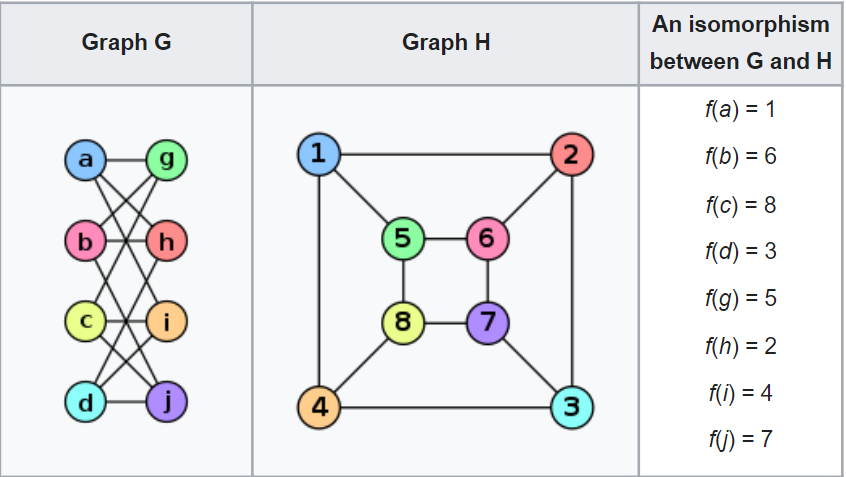
\includegraphics[width=7cm]{images/graphisomorphic.png}\\
\end{center}
Similarly in the image below, the two graphs are isomorphic as their connectivity is retained. \\
\begin{center}
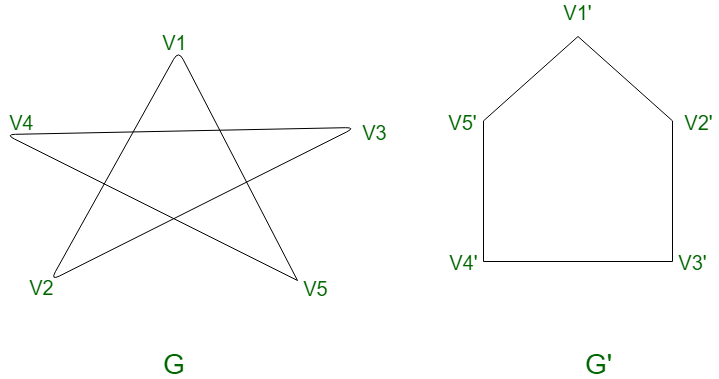
\includegraphics[width=7cm]{images/isomorphism.png}\\
\end{center}
In order to find if two graphs are isomorphic the challenge is to look for:\\
\begin{itemize}
\item Equal number of vertices \\
\item Equal number of edges\\
\item Same degree sequence\\
\item Same number of circuits of particular length\\
\end{itemize}
Hence, this problem is a NP-Intermediate problem as no current solution is known that is either NP complete or polynomial time. However for some special cases of graphs, such as trees, planar graphs and circular graphs, the problem could be solved in polynomial time. This problem has found myriad applications in computer vision, pattern recognition and graph matching. The problem is sometimes also referred as the "exact graph matching".  As a consequence of its broad application, there is a need for efficient solution. \\
\section{Algorithms/design techniques}
In our group project, our goal is to explore three different approaches to check if two graphs are isomorphic, implement and perform a comparative complexity analysis on them. The design approaches include:\\
\begin{itemize}
\item Divide and Conquer Approach\\
\item Randomized approach that would be based on quantum walks (walks on coin flips)\\
\item Brute Force Approach \\
\end{itemize}
The language that we will be using to implement and perform experimental analysis would be python however it is tentative and may subject to change. 

\begin{table}[H]
    \begin{tabular}{c c c c}
        \textbf{Algorithm} & \textbf{BestCase} & \textbf{AverageCase} & \textbf{WorstCase}  \\
        Brute Force&O($n!$)&O($n!$)&O($n!$) & \\
        VF2 & O($n^2$) & O($n!$) & O($n!n$) \\ 
        WL & O($hm$) & O($hm$) & O($hm$)
    \end{tabular}
    \caption{Complexities}
    \label{tab:my_label}
\end{table}

\begin{thebibliography}{10} % 100 is a random guess of the total number of 
%references
\addtolength{\leftmargin}{0.2in} % sets up alignment with the following line.
\setlength{\itemindent}{-0.2in}
\bibitem{b1}$https://www.tutorialspoint.com/graph_theory/graph_theory_isomorphism.htm$
\\
\bibitem{b2}$https://www.geeksforgeeks.org/mathematics-graph-isomorphisms-connectivity$
\\
\bibitem{b3}$https://dl.acm.org/doi/pdf/10.1145/3372123?casa_token=mTRtvz0gKp0AAAAA:3ngGMZ8I-pGnQmC3ALKgWwuc2cO_5wj_rk6wJEi21qwEpBqDwK14SvcGypOPFMlp2Qw2JrlfJY69jw$
\\
\bibitem{b4}$https://dl.acm.org/doi/abs/10.1145/3448016.3452820?casa_token=Bfc8gX_ri7QAAAAA:od3N91NbMQAA3lugIwi6PKa_BgV-gH9GArJUm4ZFPzwBi6s-JE_PeDTCN6m07ufUcPS5YLIpLHqwcg$
\\
\bibitem{b5}$https://api.research-repository.uwa.edu.au/ws/portalfiles/portal/1491462/10806_PID10806.pdf$

\end{thebibliography}

\end{document}
>>>>>>> Stashed changes
